\clearpage
\appendix

% =========================================================
\section{Supplementary Tables and Figures}
\label{app:figures}

This appendix gathers supporting tables and figures referred to in Sections~\ref{sec:methodology} to~\ref{sec:proposta}.

\begin{table}[!htbp]
\centering
\caption{Exclusion criteria.}
\label{tab:criteria}
\scriptsize
\begin{tabular}{|c|>{\raggedright\arraybackslash}p{10.2cm}|}
\hline
\textbf{Code} & \textbf{Criterion} \\
\hline
E1 & Duplicate record. \\
E2 & Not a peer-reviewed primary study (review, survey, editorial or preprint). \\
E3 & Outside the industrial context (e.g., healthcare, buildings, civil infrastructure, IT maintenance). \\
E4 & Only failure prediction, detection or diagnosis, with no decision component. \\
E5 & No evaluation of any kind. \\
E6 & Insufficient methodological detail. \\
E7 & Full text not accessible. \\
E8 & Maintenance management without decisions on interventions or assets (e.g., skills, barriers, KPIs). \\
E9 & The decision is not the prioritisation, selection or scheduling of interventions or assets (e.g., strategy selection, interval optimisation, joint production and maintenance scheduling). \\
E10 & Not applied to real data or an industrial case with a comparison against current practice, another method or a before/after measurement. \\
\hline
\end{tabular}
\end{table}

\begin{figure}[!htbp]
\centering
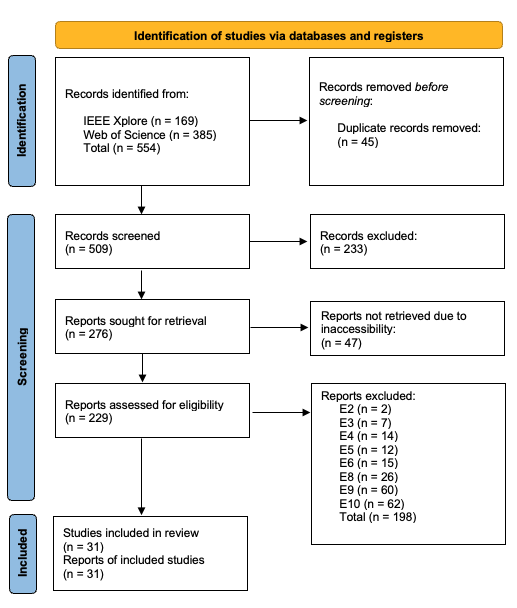
\includegraphics[width=0.7\textwidth]{figuras/prisma.png}
\caption{PRISMA 2020 flow diagram of the study selection.}
\label{fig:prisma}
\end{figure}

\begin{table}[!htbp]
\centering
\caption{Comparison of maintenance strategies.}
\label{tab:strategies}
\scriptsize
\begin{tabular}{|>{\raggedright\arraybackslash}p{1.7cm}|>{\raggedright\arraybackslash}p{2.6cm}|>{\raggedright\arraybackslash}p{2.8cm}|>{\raggedright\arraybackslash}p{3.3cm}|}
\hline
\textbf{Strategy} & \textbf{Trigger} & \textbf{Information required} & \textbf{Main limitation} \\
\hline
Corrective & Occurrence of a failure & Failure reports & Unplanned downtime and secondary damage \\
\hline
Preventive & Fixed time or usage interval & Manufacturer data, failure history & Interventions on healthy equipment \\
\hline
Condition-based & Indicator exceeds a threshold & Condition monitoring data & No anticipation of the failure time \\
\hline
Predictive & Estimated RUL & Sensor data, prognostic models & Does not define which action to take or in which order \\
\hline
Prescriptive & Recommended action and timing & Predictions, costs, resources and constraints & Requires integration of data, models and organisational knowledge \\
\hline
\end{tabular}
\end{table}

\begin{table}[!htbp]
\centering
\caption{Prioritisation criteria used in the included studies ($n$ = number of studies).}
\label{tab:criteria-use}
\scriptsize
\begin{tabular}{|>{\raggedright\arraybackslash}p{2.3cm}|>{\raggedright\arraybackslash}p{3.6cm}|>{\raggedright\arraybackslash}p{3.9cm}|c|}
\hline
\textbf{Category} & \textbf{Typical indicators} & \textbf{Studies} & $\boldsymbol{n}$ \\
\hline
Resources and operational constraints & Crews, skills, man-hours, budget, spare parts, downtime windows, travel & \cite{ozcan2021,bulut2021,panwar2021,darko2026,rios2025,rios2024,schulze2022,enjavimadar2022,moradi2024,geng2022,woller2023,gao2024,wehbi2026,wittbrodt2026,danach2026,bi2022,li2027,zhou2024,dui2025} & 19 \\
\hline
Likelihood of failure & Occurrence, failure rate, MTBF, number of past failures & \cite{ozcan2021,bulut2021,delgado2026,panwar2021,bahadir2026,gopalakrishnan2022,rios2025,enjavimadar2022,moradi2024,qiu2026,hall2021,zhou2024,danach2026,astepe2021,darko2026,dui2026} & 16 \\
\hline
Production or service impact & Downtime, bottlenecks, OEE, line efficiency, energy not supplied, SAIFI, SAIDI & \cite{yang2021,gopalakrishnan2022,panwar2021,rios2025,wittbrodt2026,danach2026,geng2022,bahrami2021,enjavimadar2022,moradi2024,shaulagara2023,zhou2024,hedayatnia2025,hall2021,dui2025,dui2026} & 16 \\
\hline
Cost & Intervention cost, downtime and interruption cost, financial risk & \cite{darko2026,schulze2022,enjavimadar2022,moradi2024,geng2022,woller2023,wittbrodt2026,danach2026,zhou2024,bahadir2026,shaulagara2023,dui2025,dui2026,bahrami2021,wehbi2026} & 15 \\
\hline
Condition, degradation and RUL & Sensor-based health indices, wear, corrosion, predicted RUL & \cite{tang2026,darko2026,schulze2022,rios2024,geng2022,hedayatnia2025,wittbrodt2026,danach2026,dui2025,bi2022,shaulagara2023,zhou2024,rios2025,wehbi2026} & 14 \\
\hline
Detectability & Detection of the failure before it causes damage & \cite{ozcan2021,bulut2021,delgado2026,panwar2021,rios2025,enjavimadar2022,moradi2024,qiu2026,hall2021} & 9 \\
\hline
Asset importance & Criticality class, importance measures, regulatory requirements & \cite{astepe2021,rios2024,hedayatnia2025,dui2025,dui2026,wittbrodt2026,moradi2024,gao2024,geng2022} & 9 \\
\hline
Safety and environment & Risk to people, explosion, environmental damage & \cite{panwar2021,bahadir2026,rios2025,delgado2026,hall2021,shaulagara2023,enjavimadar2022} & 7 \\
\hline
\end{tabular}
\end{table}

\begin{table}[!htbp]
\centering
\caption{Types of validation in the included studies ($n$ = number of studies).}
\label{tab:validation}
\scriptsize
\begin{tabular}{|>{\raggedright\arraybackslash}p{2.5cm}|>{\raggedright\arraybackslash}p{4.1cm}|>{\raggedright\arraybackslash}p{3.5cm}|c|}
\hline
\textbf{Type} & \textbf{Description} & \textbf{Studies} & \textbf{n} \\
\hline
Field implementation & Recommendations applied in the plant; indicators compared before and after & \cite{ozcan2021,bulut2021,delgado2026,hall2021,wittbrodt2026,hedayatnia2025} & 6 \\
\hline
Comparison with current practice & Proposed plan compared with the company's plan or with expert decisions on the same data & \cite{rios2025,rios2024,enjavimadar2022,moradi2024,wehbi2026,li2027,gao2024,shaulagara2023,bi2022,bahadir2026,astepe2021} & 11 \\
\hline
Comparison with other methods & Same case solved with alternative methods or policies & \cite{panwar2021,bahrami2021,qiu2026,geng2022,zhou2024,danach2026,tang2026,darko2026} & 8 \\
\hline
Simulation or benchmark & Simulation model of the real system or public benchmark instances & \cite{yang2021,gopalakrishnan2022,dui2025,dui2026,schulze2022,woller2023} & 6 \\
\hline
\end{tabular}
\end{table}

\begin{table}[!htbp]
\centering
\caption{Comparison of the families of approaches found in the included studies.}
\label{tab:families}
\scriptsize
\begin{tabular}{|>{\raggedright\arraybackslash}p{1.6cm}|>{\raggedright\arraybackslash}p{3.1cm}|>{\raggedright\arraybackslash}p{3.3cm}|>{\raggedright\arraybackslash}p{2.4cm}|}
\hline
\textbf{Family} & \textbf{Strengths} & \textbf{Limitations} & \textbf{Studies} \\
\hline
MCDM & Transparent; uses expert knowledge; needs no sensor data & Static ranking; subjective weights; compensatory aggregation; resources only when combined with optimisation & \cite{ozcan2021,bulut2021,panwar2021,bahrami2021,enjavimadar2022,moradi2024,rios2025} \\
\hline
Risk and FMEA & Familiar to maintenance teams; consistent with RCM; links severity and likelihood & Ordinal scores; ranks risks rather than interventions; resources rarely considered & \cite{bahadir2026,qiu2026,shaulagara2023,zhou2024,hedayatnia2025} \\
\hline
Hybrid with ML & Uses condition data; can be updated as new data arrive & Needs large labelled histories; labels are proxies or past decisions; predictive part hard to explain & \cite{tang2026,darko2026,astepe2021,wehbi2026,danach2026,rios2024,wittbrodt2026} \\
\hline
Optimisation and scheduling & Handles crews, budgets and time windows; scales to large instances & Priorities given a priori or hidden in costs; many assumed parameters; metaheuristics and DRL hard to explain & \cite{schulze2022,geng2022,woller2023,gao2024,bi2022,dui2025,dui2026,li2027} \\
\hline
Simulation and industrial practice & Grounded in production impact; implemented in real plants & Specific to one line or plant; hard to generalise; evaluation without control & \cite{yang2021,gopalakrishnan2022,delgado2026,hall2021} \\
\hline
\end{tabular}
\end{table}

\begin{table}[!htbp]
\centering
\caption{Functional and non-functional requirements of the proposed system.}
\label{tab:requirements}
\scriptsize
\begin{tabular}{|p{0.9cm}|>{\raggedright\arraybackslash}p{9.0cm}|c|}
\hline
\textbf{ID} & \textbf{Requirement} & \textbf{Gap} \\
\hline
FR01 & Import pending interventions, equipment data and work orders (e.g., from CSV files or a CMMS). & -- \\
FR02 & Estimate the failure probability of each asset from its condition data. & -- \\
FR03 & Let each stakeholder define the importance of the criteria through pairwise comparisons, warn when judgements are inconsistent (\textit{CR} $\geq 0.1$) and aggregate the judgements of all stakeholders. & G4, G5 \\
FR04 & Place every intervention with a safety risk at the top of the list, regardless of the other criteria. & G1 \\
FR05 & Rank the remaining pending interventions and recompute the ranking when new data or failures arrive. & G3 \\
FR06 & Explain each position by showing the contribution of each criterion. & G5 \\
FR07 & Show how the ranking changes when the weights are changed (sensitivity analysis). & G4 \\
FR08 & Store each ranking, the decision taken and, later, its outcome. & G6 \\
\hline
NFR01 & Performance: produce the ranking in a few seconds for a few hundred interventions. & -- \\
NFR02 & Usability: be understandable by users without knowledge of MCDM methods. & -- \\
NFR03 & Transparency: no recommendation is shown without its justification. & G5 \\
NFR04 & Interoperability: import data in common formats and allow connection to a CMMS. & -- \\
NFR05 & Security: require authentication, with separate profiles for managers and other users. & -- \\
\hline
\end{tabular}
\end{table}

\begin{figure}[!htbp]
\centering
\begin{tikzpicture}[
  font=\scriptsize,
  box/.style={draw, rounded corners=2pt, align=center, minimum height=0.95cm, text width=1.95cm},
  src/.style={draw, dashed, align=center, minimum height=0.6cm, text width=1.95cm},
  arr/.style={-{Stealth[length=2mm]}, thick}
]
\node[src] (sources) at (0,0) {Sensors, work orders, costs, stock};
\node[box] (data)  at (2.45,0) {\textbf{Data module}\\ cleaning,\\ integration};
\node[box] (pred)  at (4.9,0) {\textbf{Predictive module}\\ failure\\ probability (ML)};
\node[box] (dec)   at (7.35,0) {\textbf{Decision module}\\ 1.\ safety constraint\\ 2.\ TOPSIS ranking};
\node[box] (ui)    at (9.8,0) {\textbf{Interface}\\ ranking,\\ explanation,\\ what-if};
\node[src] (stake) at (4.9,-2.2) {Maintenance, production, safety staff};
\node[box] (w)     at (7.35,-2.2) {\textbf{Weighting module}\\ AHP, consistency, aggregation};
\draw[arr] (sources) -- (data);
\draw[arr] (data) -- (pred);
\draw[arr] (pred) -- (dec);
\draw[arr] (dec) -- (ui);
\draw[arr] (stake) -- (w);
\draw[arr] (w) -- (dec);
\draw[arr, dashed] (ui.north) -- ++(0,0.55) -| node[pos=0.25, above] {decision history} (data.north);
\end{tikzpicture}
\caption{Conceptual architecture of the proposed system.}
\label{fig:arquitetura}
\end{figure}

% =========================================================
\section{Exploratory Analysis of the Dataset}
\label{app:eda}

This appendix characterises the Microsoft Azure Predictive Maintenance dataset described in Section~\ref{sec:dataset}. The analysis was carried out in Python with pandas and matplotlib.

\paragraph{Structure and quality.} The dataset is split into five files (Table~\ref{tab:dataset}). All 100 machines have a complete hourly telemetry series for 2015 (8,761 records each), and no file contains missing values or duplicated rows. The maintenance file also includes 400 replacements from 2014, which provide the history needed to compute the time since the last replacement at the start of 2015. Of the 761 failures, 743 match a replacement in the maintenance file; the remaining 18 all occur on 2 January 2015 at 03:00 and are an artefact of the start of the series rather than missing records. Failures account for 25.7\% of the 2,886 replacements made in 2015, so about three quarters of the interventions are preventive.

\begin{table}[!htbp]
\centering
\caption{Files of the Microsoft Azure Predictive Maintenance dataset.}
\label{tab:dataset}
\scriptsize
\begin{tabular}{|l|r|>{\raggedright\arraybackslash}p{7.6cm}|}
\hline
\textbf{File} & \textbf{Records} & \textbf{Content} \\
\hline
Telemetry & 876,100 & Hourly mean of voltage, rotation, pressure and vibration per machine, 1 January 2015 to 1 January 2016 \\
Errors & 3,919 & Non-critical errors of five types (error1--error5), with timestamp and machine \\
Maintenance & 3,286 & Component replacements (comp1--comp4), scheduled or after failure, June 2014 to December 2015 \\
Failures & 761 & Replacements caused by a failure, by component, in 98 of the 100 machines \\
Machines & 100 & Model (model1--model4) and age in years (0--20) \\
\hline
\end{tabular}
\end{table}

\paragraph{Sensor distributions.} The four sensors follow approximately symmetric, bell-shaped distributions (Fig.~\ref{fig:eda-sensors}), with means of 170.8 (voltage), 446.6 (rotation), 100.9 (pressure) and 40.4 (vibration). The correlation between any two sensors is close to zero, so each carries independent information. Extreme readings are concentrated before failures: between 18\% and 26\% of the readings more than three standard deviations from the mean fall in the 48 hours that precede a failure, although these periods cover only 4\% of the data.

\begin{figure}[!htbp]
\centering
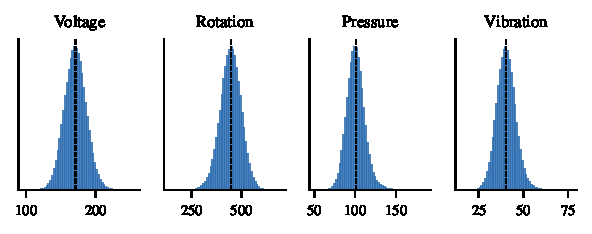
\includegraphics[width=\textwidth]{figuras/eda_sensors.pdf}
\caption{Distribution of the hourly sensor readings (dashed line: mean).}
\label{fig:eda-sensors}
\end{figure}

\paragraph{Failures by component and machine model.} Component~2 fails most often (259 failures) and component~3 least often (131). Model~3 and model~4 account for two thirds of the fleet, but model~1 and model~2 machines fail about twice as often per machine (Fig.~\ref{fig:eda-failures}). The median interval between two failures of the same component in the same machine is 75 days. Monthly failures are stable, between 50 and 69, except for January, which is inflated by failures recorded on the first day of the series.

\begin{figure}[!htbp]
\centering
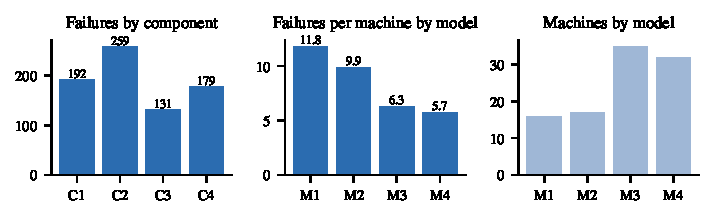
\includegraphics[width=\textwidth]{figuras/eda_failures.pdf}
\caption{Failures by component, failures per machine by model, and number of machines by model.}
\label{fig:eda-failures}
\end{figure}

\paragraph{Behaviour before failure.} Fig.~\ref{fig:eda-signature} shows, for each component, the deviation of one sensor from its overall mean in the 96 hours before a failure. Each component is associated with a different sensor, and the deviation appears abruptly about 48 hours before the failure: voltage rises by about 12\% before failures of component~1, rotation falls by about 17\% for component~2, pressure rises by about 24\% for component~3 and vibration rises by about 25\% for component~4. This pattern supports a classifier based on rolling sensor statistics over the last 24 to 48 hours. At the same time, only 1.96\% of machine-hours precede a failure within 24 hours, so the training will have to handle a strong class imbalance.

\begin{figure}[!htbp]
\centering
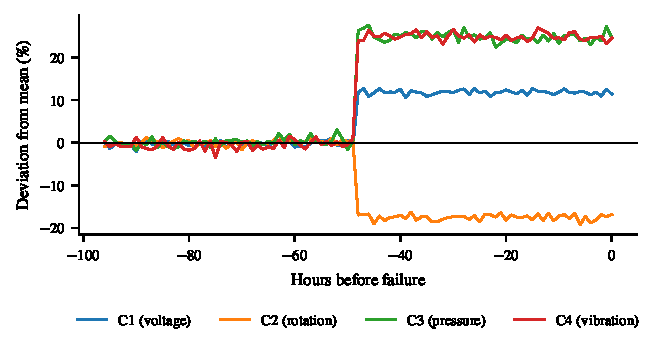
\includegraphics[width=\textwidth]{figuras/eda_signature.pdf}
\caption{Mean deviation of the associated sensor from its overall mean before failures of each component.}
\label{fig:eda-signature}
\end{figure}

\paragraph{Machine age and errors.} The number of failures per machine grows with machine age ($r = 0.47$) and with the number of errors recorded during the year ($r = 0.54$), as shown in Fig.~\ref{fig:eda-age}. Errors are therefore useful as an early indicator, even though they do not stop the machine, and age and model can serve as measures of asset importance in the ranking.

\begin{figure}[!htbp]
\centering
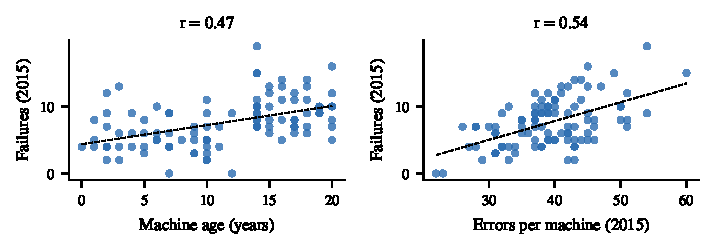
\includegraphics[width=\textwidth]{figuras/eda_age_errors.pdf}
\caption{Failures per machine in 2015 against machine age and against the number of errors.}
\label{fig:eda-age}
\end{figure}

\paragraph{Implications for the prototype.} The dataset provides what the predictive module needs: a clear signal before failures, an identifiable set of assets and components, and a maintenance history. It does not provide costs, intervention durations, production impact or safety information, which will be added as assumptions. Since the data are simulated, the prototype will demonstrate the behaviour of the system rather than its effect on a real plant.